\documentclass[../main.tex]{subfiles}

\begin{document}

\section{Overview}

Identifying groups of patients meeting a given set of eligibility criteria is a critical step for recruitment into randomized controlled trials (RCTs). Often, clinical studies fall short of recruitment goals, leading to time and cost overruns or  challenges in ensuring adequate statistical power \cite{gul2010clinical, adams2015barriers}. Failure to recruit research subjects may result from a variety of factors, but often stems from difficulties in translating complex eligibility criteria into effective queries that can sift through data  in the electronic health record (EHR) \cite{wang2017classifying}. Despite these difficulties, RCT investigators  increasingly rely on EHR data queries to  identify research candidates instead of labor-intensive manual chart or case report form review \cite{cowie2017electronic}. At the same time, the amount and variety of data contained in EHRs is increasing dramatically, creating both challenges and opportunities for patient recruitment \cite{lee2017medical}. While more granular and potentially useful data are captured and stored in EHRs now than in the past, the process of accessing and leveraging that data requires technical expertise and extensive knowledge of biomedical terminologies and data models. 

Cohort discovery tools such as Leaf \cite{dobbins2019leaf} and i2b2 \cite{murphy2010serving} may be used in many situations, as they offer relatively simple drag-and-drop interfaces capable of querying EHR data to find patients meeting given criteria \cite{johnson2014use}.  However, these tools have limitations, since their use often requires significant training  and the tools have difficulty representing particularly complex nested or temporal eligibility criteria \cite{deshmukh2009evaluating}. Moreover, existing cohort discovery tools lack functionality to dynamically reason upon non-specific criteria that frequently appear in real-world eligibility criteria. For example, a criterion may require patients "indicated for bariatric surgery", but translating such non-specific criteria into a query (e.g., patients with a diagnosis of morbid obesity or body mass index greater than 40) must be performed manually by a researcher, even in cases where constructing an exhaustive list of such criteria may be time-intensive, subjective, and error-prone. 

In recent years, alternatives to web-based cohort discovery tools have been explored. In particular, various methods using Natural Language Processing (NLP) have been put forth by the research community \cite{yuan2019criteria2query, soni2020patient, fang2022combining, zhang2020deepenroll, chen2019clinical, patrao2015recruit, dhayne2021emr2vec, liu2021evaluating, xiong2019cohort}. NLP-based cohort discovery methods could be especially valuable since they can key on eligibility criteria described in natural language, a medium that clinicians,  researchers and investigators already use.

\section{Related Work}

Various methods for cohort discovery using NLP have been previously explored. Yuan \textit{et al} developed Criteria2Query \cite{yuan2019criteria2query}, a hybrid information extraction (IE) pipeline and application which uses both rules and machine learning to generate database queries on an Observation Medical Outcomes Partnership (OMOP) \cite{hripcsak2015observational} database, later expanded by Fang \textit{et al} \cite{fang2022combining}. Other research has used encoder-decoder neural architectures for transforming clinical natural language questions into SQL queries \cite{bae2021question, park2021knowledge, wang2020text, pan2021bert, dhayne2021emr2vec}. These studies include exploration of cross-domain transformations, where systems must generalize to unseen database schema \cite{park2021knowledge}, handling of typos and abbreviations \cite{bae2021question}, and the generation of intermediate representations between a natural language utterance and final SQL database query.\cite{pan2021bert} 

Beyond database query generation, other cohort discovery methods explored include document ranking and classification \cite{chen2019clinical,soni2020patient} where clinical notes are summarized, ranked and classified as relevant to a given eligibility criterion, and embedding projections for entailment prediction \cite{dhayne2021emr2vec, zhang2020deepenroll} where predicting that a patient can be inferred from a given eligibility criteria equates to eligibility. Other studies have explored the use of ontologies and OWL-based reasoning in determining eligibility \cite{patel2007matching, huang2013semanticct, baader2018patient, johnson2016mimic, patrao2015recruit}.
    
\subsection{Gaps and opportunities}

To date, most programs capable of generating database queries do so for only a single database schema, such as OMOP or MIMIC-III \cite{johnson2016mimic}. This lack of flexibility limits their capability to accommodate real-world project needs \cite{belenkaya2021extending, peng2021towards, zoch2021adaption, warner2019hemonc, zhou2013evaluation, shin2019genomic, kwon2019development}, such as adding new database tables to OMOP for cancer staging \cite{belenkaya2021extending}. Moreover, most methods, particularly those using direct text-to-SQL deep learning approaches, tend to generate relatively simple SQL statements with few JOINs or nested sub-queries and typically no support for UNION operators and so on. This relative simplicity contrasts with the complexity of real-world EHR databases, which may contain dozens or even hundreds of tables using various vocabularies and mappings. Furthermore, direct text-to-SQL methods are bound to SQL syntax, and thus incapable of querying other systems such as Fast Healthcare Interoperability Resources (FHIR) \cite{bender2013hl7}. Additionally, few of the methods described provide support for complex logic such as nested Boolean statements or temporal sequences, and none support reasoning on non-specific criteria (e.g., "diseases that affect respiratory function"), phenomena common to study eligibility criteria \cite{wang2017classifying, ross2010analysis}. Perhaps most importantly, to the best of our knowledge, only one previous work has been tested in terms of matching patients actually enrolled in clinical trials \cite{zhang2020deepenroll}, and none have been directly compared to the capabilities of a human database programmer.

\subsection{Key Contributions}

We introduce the LeafAI query engine, an application capable of generating database queries for cohort discovery from free-text eligibility criteria. This work contributes the following:

\begin{enumerate}
    \item{A novel database annotation schema and mapping method to enable \textbf{data model-agnostic} query generation from natural language.}
    \item{Methods for transforming and leveraging \textbf{intermediate logical representations} of eligibility criteria.}
    \item{A \textbf{corpus of human-annotated logical forms of eligibility criteria} available to the research community.}
    \item{Methods for dynamically \textbf{reasoning upon non-specific criteria} using an integrated knowledge base (KB) of biomedical concepts.}
    \item{An evaluation of system performance by \textbf{direct comparison to that of a human database programmer} on actual clinical trial enrollments}.
\end{enumerate}

\section{Methods}

\subsection{System Architecture}

The LeafAI query engine was designed using a modular, micro service-based architecture with a central Application Program Interface (API) which orchestrates end-to-end query generation. Inter-module communication is performed using gRPC \cite{grpc}, a robust open-source remote procedure call framework which enables language-agnostic service integration. This allows individual modules to be implemented (and substituted) in programming languages and using libraries well-suited to a given task. A diagram of the LeafAI query engine architecture is shown in Figure \ref{fig_leafai_architecture}. 

\begin{figure}[h]
  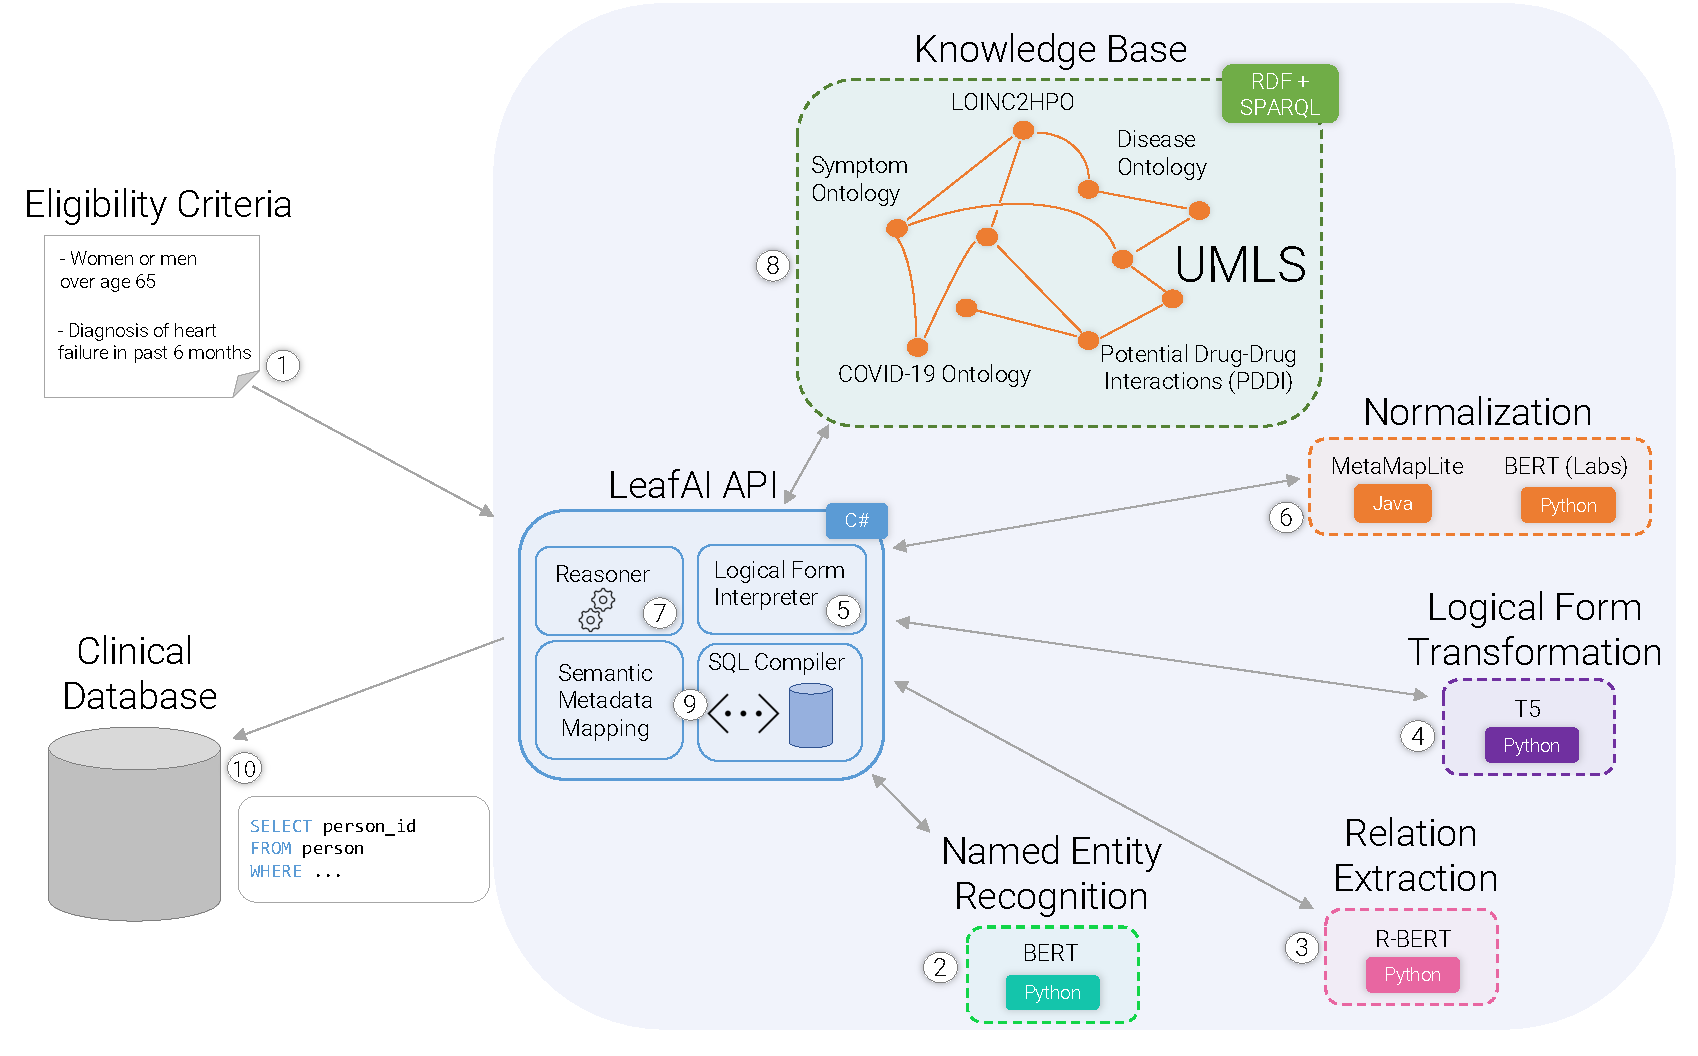
\includegraphics[scale=0.57]{Figures/7_query_generation/leafai_architecture.pdf}  
\caption{LeafAI query architecture. Inter-module communication is performed using the gRPC framework. Individual modules are deployed as Docker \cite{docker} containers and communicate solely with the central API, which orchestrates query generation and handles query generation requests.}
\label{fig_leafai_architecture}
\end{figure}

At a high level, query generation is performed in the following steps:

\begin{enumerate}
    \item{A query request is received by the API in the form of inclusion and exclusion criteria as free-text strings.}
    \item{The input texts are tokenized and named entity recognition is performed to determine spans of text representing conditions, procedures, and so on.}
    \item{Relation extraction is performed to determine relations between the entities, such as \textit{Caused-By} or \textit{Numeric-Filter}.}
    \item{The input texts are transformed by replacing spans of "raw" text with logical form names. For example, "Diagnosed with diabetes" would become "Diagnosed with cond("diabetes")." The resulting input texts are in turn transformed into an output logical representation using a Sequence to Sequence (Seq2Seq) architecture, in the form of a string.}
    \item{A logical form interpreter module implemented as a recursive descent parser \cite{johnstone1998generalised} reads the logical form string input and instantiates it as an abstract syntax tree (AST) of nested in-memory logical form objects.}
    \item{"Named" logical form objects (i.e., specified with quoted text, such as "cond("diabetes")") are normalized into one or more corresponding UMLS concepts. UMLS child concepts are also added using our KB. For example, "cond("type 2 diabetes")” would also include concepts for type 2 diabetes with kidney complications (C2874072).}
    \item{Working recursively inside-to-outside the AST structure, each logical form object calls a \textit{Reason()} method which executes various rules depending on context.}
    \item{Each reasoning rule is performed as one or more pre-defined SPARQL queries to the KB, concept by concept.}
    \item{The final normalized, reasoned, logical form AST is thus a nested structure of UMLS concepts. Each AST criterion is mapped to zero or more corresponding entries in the semantic metadata mapping (SMM), which in turn lists meanings, roles, and relations of a database schema in the form of UMLS concepts.}
    \item{The final mapped AST object is transformed into a series of database queries, one per line of eligibility criteria text. The output SQL query can either be executed directly on a database or returned to the API caller.}
\end{enumerate}

\noindent Figure \ref{fig_leafai_querygen} illustrates an example of this process. In the following subsections we examine these steps in detail.

\begin{figure}[h]
  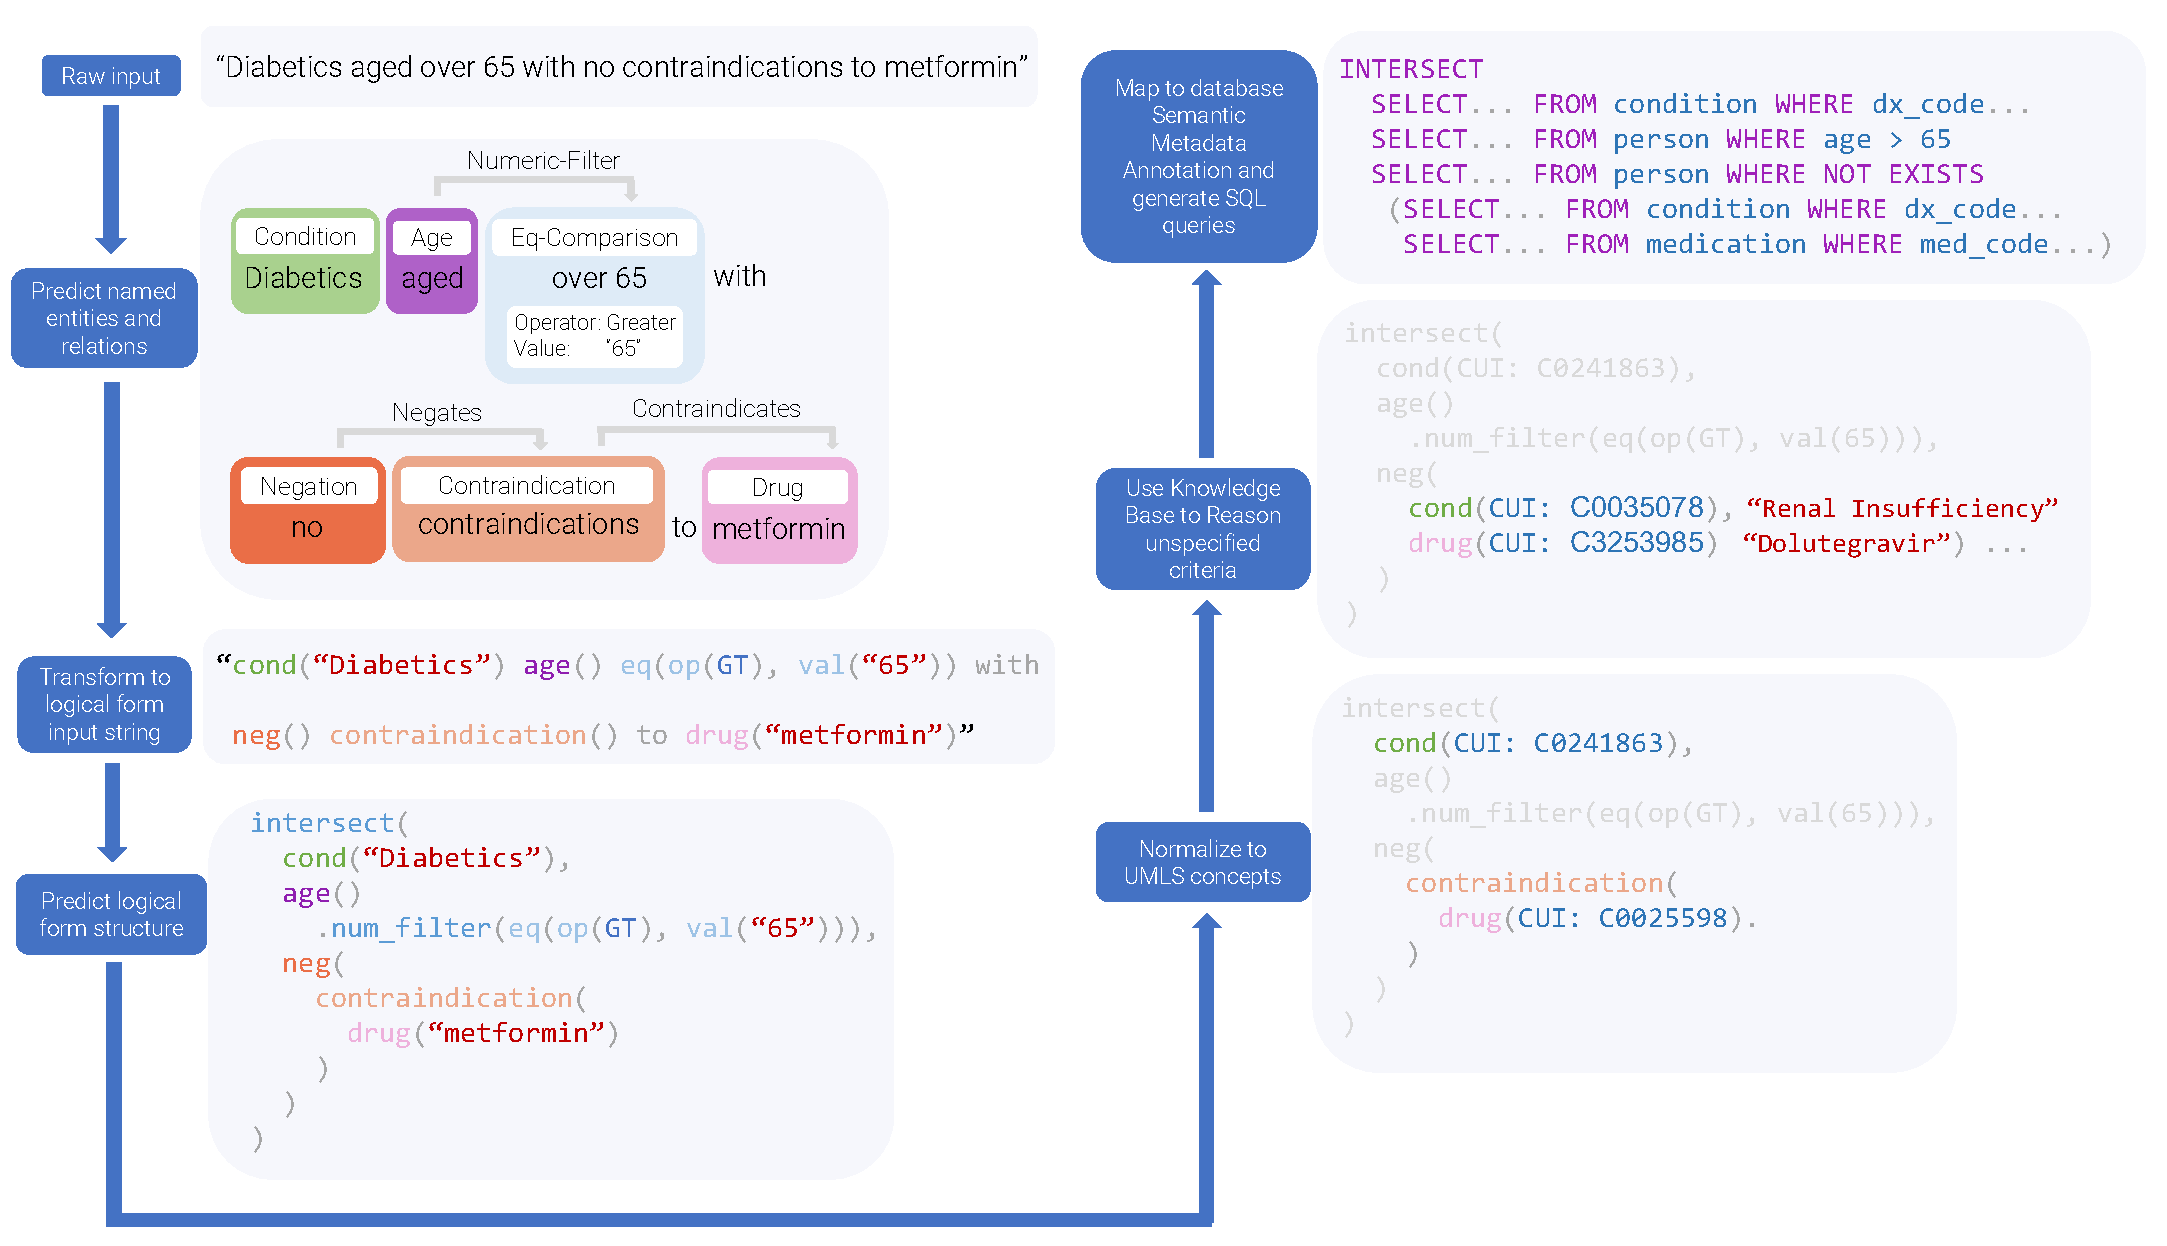
\includegraphics[scale=0.46]{Figures/7_query_generation/leafai_flow.pdf}  
\caption{LeafAI query generation processes}
\label{fig_leafai_querygen}
\end{figure}

\subsection{Named entity recognition and relation extraction}

\noindent Named entity recognition (NER) refers to the segmentation and identification of tokens within an input sentence as "entities", such as conditions or procedures. We used the Leaf Clinical Trials (LCT) corpus \cite{dobbins2022leaf} to train two BERT-based \cite{devlin2018bert} NER extractors, one each for LCT general- and fine-grained-entities (see \cite{dobbins2022leaf} for more information on LCT entity types). Next, we perform relation extraction between named entity pairs similarly using a BERT-based model also trained on the LCT corpus.

\subsection{Logical form transformation}

One of the core challenges of generating queries for eligibility criteria is the problem of logical representation. Generating queries directly based on named entities and relations alone, while practical, performs poorly in cases of nested or particularly complex logic. An alternative to this approach is to use a so-called intermediate representation (IR), which transforms the original natural language by removing "noise" unnecessary to a given task and which more logically represents underlying semantics (see Herzig \textit{et al} \cite{herzig2021unlocking} for an examination of IR-based SQL generation approaches). Similar to earlier work using Description Logics, Roberts and Demner-Fushman \cite{roberts2016annotating} proposed a representation of questions on EHR databases using a comparatively compact but flexible format using first order logic expressions, for example, representing "Is she wheezing this morning?" as

\begin{quote}
    \centering
    $\delta( \lambda x.has\_problem(x, C0043144, status) \wedge time\_within(x, \mathrm{"this\ morning"}))$
\end{quote}

\noindent This style of representation is powerfully generalizable, but also difficult to translate directly into SQL statements as multiple predicates (e.g., \textit{has\_problem} and \textit{time\_within}) may actually correspond to one or many SQL statements, depending on context, complicating direct transformation into queries.

We thus chose a similar intermediate representation (hereafter simply "logical forms") as proposed by Roberts and Demner-Fushman but more closely resembling a nested functional structure in programming languages such as Python or JavaScript and more amenable to SQL generation. A criterion such as "Diabetic women and men over age 65" would be represented by our logical forms as

\begin{quote}
$intersect( \\
    \mathrm{\ \ \ \ }cond("Diabetic"), \\
    \mathrm{\ \ \ \ }union(female(), male()),\\
    \mathrm{\ \ \ \ }age().num\_filter(eq(op(GT), val("65"))) \\
)$
\end{quote}

After NER and relation extraction are performed, we leverage T5 \cite{raffel2020exploring}, a state-of-the-art Seq2Seq architecture we fine-tuned for predicting logical forms on the LLF corpus. As inputs to the Seq2Seq model we use the original eligibility criteria with named entity spans replaced by logical form representations, since we found this improved performance compared to training with raw inputs. Thus the above example input would be transformed to

\begin{quote}
    \centering
    $\textit{"cond(“Diabetic”) female() and male() over age() eq(op(GT), val(“65”))"}$
\end{quote}

\noindent The returned logical form string is then instantiated into an abstract syntax tree (AST) of nested in-memory logical form objects using a recursive descent parser \cite{johnstone1998generalised} within our API.

\subsection{Concept normalization}

Normalization refers to the mapping of free-text string values (e.g., "diabetes mellitus") to coded representations (e.g., UMLS, ICD-10, SNOMED, or LOINC). We normalize "named" logical forms to UMLS concepts using MetaMapLite \cite{aronson2001effective, demner2017metamap}. We consider a logical form "named" if it contains a free-text value surrounded by quotes. For example, \textit{cond()} is unnamed and refers to any condition or disease, while \textit{cond("hypertension")} is named as it refers to a specific condition. 

Normalization using MetaMapLite can often result in high recall but low precision, as MetaMapLite has no NER component and tends to return UMLS concepts which match a given phrase syntactically but refer to abstract concepts not of interest (e.g., a search for "BMI" may return "body mass index" (C1305855), but also organic chemical "BMI 60" (C0910133)). To improve normalization precision, we employ two strategies. First, our NER component filters predicted UMLS concepts to only those of specific semantic types. For example, we limit condition concepts to only those related to semantic types of diseases or syndrome (dsyn) and so on. Next, using term-frequencies pre-computed across UMLS concept phrases, we compare term frequency-inverse document frequency (tf-idf) on MetaMapLite predictions, removing UMLS concepts whose summed matched spans have a tf-idf score lower than that of unmatched spans in a given named entity. For example, for the string "covid-19 infection", MetaMapLite predicts both "COVID-19" (C5203670) as well as several concepts related to general infections. Our tf-idf strategy removes general infection concepts because “infection” has a lower tf-idf score than the summed scores for “covid” + “-” + “19”. 

Laboratory values present a particular challenge, as LeafAI expects predicted lab concepts to have directly associated LOINC codes, while MetaMapLite typically normalizes lab test strings to UMLS concepts of semantic type "laboratory test or finding", but which do not have direct mappings to LOINC codes. For example, a search for "platelet count" returns the concept "Platelet Count Measurement" (C0032181), but not the needed concept of "Platelet \# Bld Auto" (C0362994) with LOINC code “777-3”. Thus similar to Lee and Uzuner with medications \cite{lee2020normalizing}, we trained a BERT model for sequence classification to normalize lab tests. We trained this model to identify UMLS concepts associated with LOINC codes most frequently used in eligibility criteria \cite{rafee2022elapro}, with each CUI as a possible class.

\subsection{Reasoning using an integrated knowledge base}

For reasoning and derivation of ICD-10, LOINC, and other codes for UMLS concepts, we designed a KB accessible via SPARQL queries and stored as Resource Description Framework (RDF) \cite{manola2004rdf} triples. The core of our KB is the UMLS, derived using a variation of techniques created for ontologies in BioPortal \cite{noy2009bioportal}. To further augment the UMLS, we mapped and integrated the Disease Ontology \cite{schriml2012disease}, Symptom Ontology \cite{sayers2010database}, COVID-19 Ontology \cite{sargsyan2020covid}, Potential Drug-Drug Interactions \cite{ayvaz2015toward}, LOINC2HPO \cite{zhang2019semantic}, and the Disease-Symptom Knowledge Base \cite{wang2008automated}. We then developed SPARQL queries parameterized by UMLS concepts for various scenarios which leveraged our KB, such as contraindications to treatments, symptoms of diseases, and so on. Using LOINC2HPO mappings further allows us to infer phenotypes by lab test results rather than using ICD-10 or SNOMED codes alone. 

Our KB, nested logical forms, and inside-to-outside normalization methods enable "multi-hop" reasoning on eligibility criteria over several steps. For example, given the non-specific criterion "Contraindications to drugs for conditions which affect respiratory function", our system successfully reasons that (among other results),

\begin{enumerate}
    \item \textbf{Asthma} causes changes to \textbf{respiratory function}
    \item \textbf{Methylprednisolone} can be used to treat \textbf{asthma}
    \item \textbf{Mycosis} (fungal infection) is a contraindication to \textbf{methylprednisolone}
\end{enumerate}

\noindent These features allow LeafAI to reason upon fairly complex non-specific criteria.

\subsection{Query generation using semantic metadata mapping}

To enable data model-agnostic query generation, we leveraged a subset of codes within the UMLS in what we define as a semantic metadata mapping, or SMM. An SMM includes a listing of available databases, tables, columns, and so on within a given database schema. Critically, these database artifacts are "tagged" using UMLS concepts. An example of this can be seen in Figure \ref{fig_leafai_smm}, which shows strategies by which a given criterion can be used to generate schema-specific queries by leveraging different SMMs. In cases where the LeafAI query engine finds more than one means of querying a concept (e.g., two SQL tables for diagnosis codes), the queries are combined in a UNION statement.

\section{Experiment Setup}

It is reasonable to expect that an NLP-based system for finding patients based on eligibility criteria would find many  patients who actually enrolled in a real clinical trial — assuming  that patients enrolled in those trials met the necessary criteria as determined by study investigators. While there are caveats to this approach (for example, certain diagnosis codes may be missing for some patients, etc.), we suggest that tools such as LeafAI be evaluated by their ability to handle real-world eligibility criteria and clinical data. 

In this study we compared LeafAI's results to that of a human database programmer experienced in the use of clinical databases and data extraction. Our evaluation was performed as follows:

\begin{enumerate}
    \item We extracted metadata on 168 clinical trials from our EHR between January 2017 and December 2021 where at least 10 patients were indicated as enrolled and not withdrawn, and the total number of raw lines within the eligibility criteria (besides the phrases "Inclusion Criteria" and "Exclusion Criteria") was less than or equal to 30.
    \item By manual review, we excluded 22 trials with multiple sub-groups, as it would not be possible to know which eligibility criteria applied to which sub-group of enrolled patients.
    \item To narrow the scope of our evaluation, we chose to evaluate only trials studying the following 7 disease groups: Cardiology, COVID-19, Crohn's Disease, Multiple Sclerosis (MS), Diabetes Mellitus, Hepatitis C, and Cancer. Using the "condition" field for each trial within metadata from \url{https://clinicaltrials.gov}, we filtered and grouped the remaining 146 trials into only those studying our diseases of interest. 
    \item We randomly chose 1 trial from each group, with the exception of Cancer, where given the large number of trials and variety of cancer types, we chose 2 trials. 427 patients were enrolled across the chosen 8 clinical trials.
    \item Both the LeafAI query engine and human programmer created queries to find patients for each eligibility criteria, which we executed on an OMOP database derived from our EHR of our institution's entire research-eligible patient population. 
    \item To ensure results returned would be limited to only data available during the time of each trial, we replaced references to the SQL function for generating a current timestamp (\textit{GETDATE()}) with that of each trial's end date, and similarly replaced OMOP table references with SQL views filtering data to only that existing prior to the end of a trial.
    \item To ensure queries would be comparable to LeafAI, the human programmer was instructed to (1) ignore criteria which cannot be computed, (2) make a best effort to reason upon non-specific criteria (e.g., symptoms for a condition), (3) not check whether patients found by a human query enrolled within a trial, and (4) skip criteria which cause an overall query to find no eligible patients.
\end{enumerate}

\section{Results}

Results of the query generation experiment are shown in Table \ref{tbl_results}. Overall, LeafAI matched 212 of 427 (49\%) total enrolled patients across 8 clinical trials compared to 180 (42\%) found by queries of the human programmer. The mean per-trial percent of patients matched was 43.5\% for LeafAI and 27.2\% for the human programmer. LeafAI had a greater number of patients deemed eligible across all 8 trials, for a total of 27,225 eligible compared to 14,587 found by the human programmer. 

\begin{table}[h!]
    \small
    \centering
    
\documentclass[../main.tex]{subfiles}

\begin{document}

Results of our evalution are shown in Table \ref{tbl_results}.

\begin{table}[h!]
    \small
    \centering
    
\documentclass[../main.tex]{subfiles}

\begin{document}

Results of our evalution are shown in Table \ref{tbl_results}.

\begin{table}[h!]
    \small
    \centering
    
\documentclass[../main.tex]{subfiles}

\begin{document}

Results of our evalution are shown in Table \ref{tbl_results}.

\begin{table}[h!]
    \small
    \centering
    \input{tables/results}
    \caption{}
    \label{tbl_results}
\end{table} 

\begin{figure}[h!]
  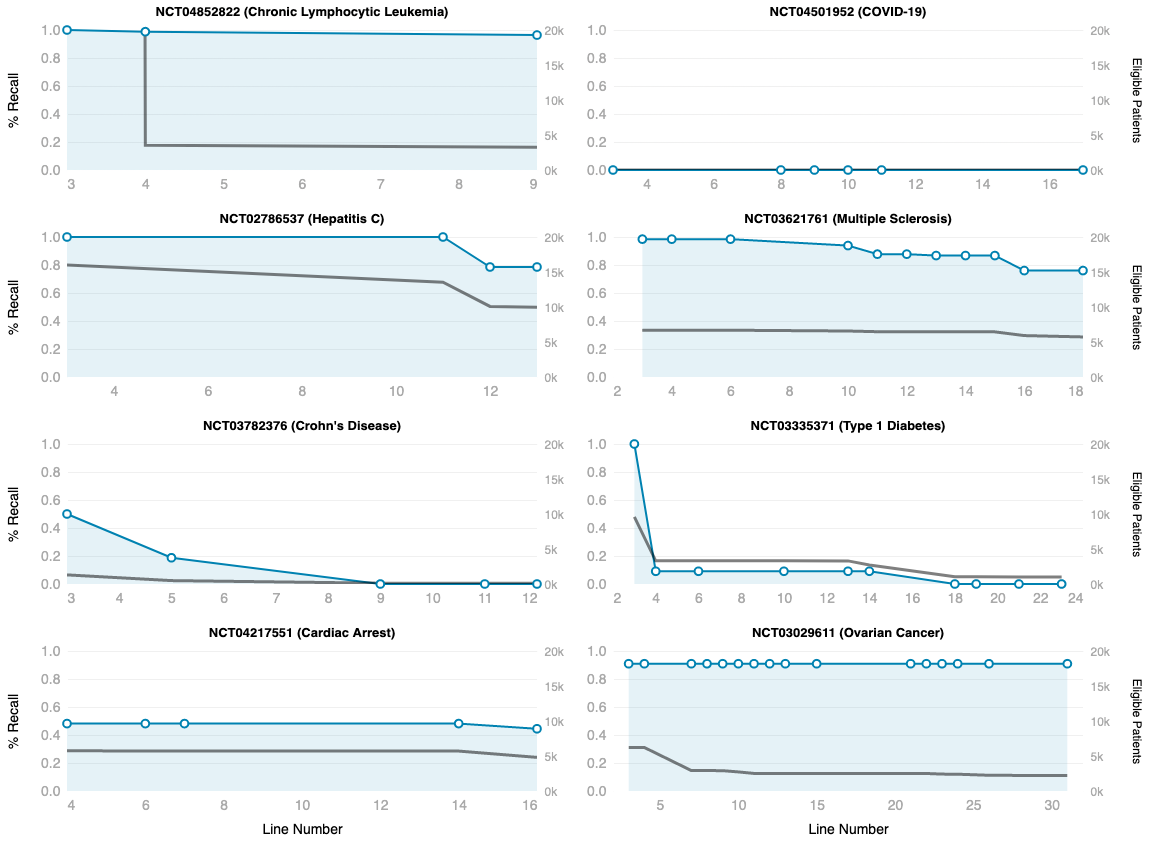
\includegraphics[scale=0.42]{figures/leafai_detail_results_longitudinal.png}  
\caption{}
\label{fig_leafai_results_longitudinal}
\end{figure}

\begin{table}[h!]
    \small
    \centering
    \input{tables/results_leafai_detail}
    \caption{}
    \label{tbl_results_leafai_detail}
\end{table} 


\end{document}
    \caption{}
    \label{tbl_results}
\end{table} 

\begin{figure}[h!]
  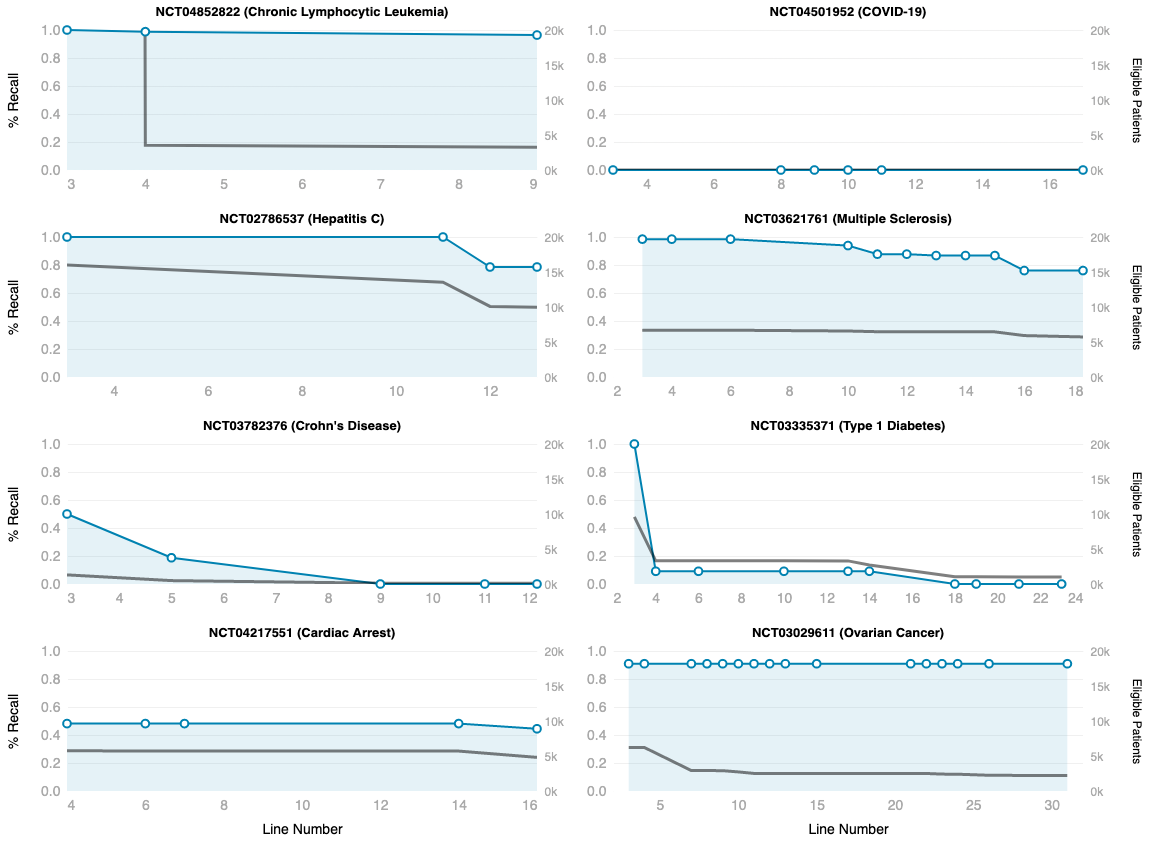
\includegraphics[scale=0.42]{figures/leafai_detail_results_longitudinal.png}  
\caption{}
\label{fig_leafai_results_longitudinal}
\end{figure}

\begin{table}[h!]
    \small
    \centering
    \def\arraystretch{1.4}
\begin{tabular}{l c c c c}
    \textbf{Condition} & \textbf{\# Criteria} & \textbf{Skipped - \newline No Patients} & \textbf{Skipped - \newline Not Computable} & \textbf{Fully Executed} \\
    \toprule
    Cl Lymphoma        & 4  & 0 (0\%)    & 0 (0\%)    & 4  (100\%)  \\
    Hepatitis C        & 8  & 0 (0\%)    & 4 (50\%)   & 4  (50\%)   \\
    Crohn's Disease    & 9  & 0 (0\%)    & 4 (44.4\%) & 5  (55.5\%) \\
    Cardiac Arrest     & 12 & 0 (0\%)    & 8 (66.6\%) & 4  (33.3\%) \\
    COVID-19           & 13 & 0 (0\%)    & 6 (46.1\%) & 7  (53.8\%) \\
    Multiple Sclerosis & 14 & 1 (7.1\%)  & 3 (21.4\%) & 10 (71.4\%) \\
    Type 1 Diabetes    & 18 & 2 (11.1\%) & 8 (44.4)   & 8  (44.4\%) \\
    Ovarian Cancer     & 25 & 2 (8\%)    & 9 (36\%)   & 14 (56\%)   \\
    \bottomrule
    \textbf{Total} & 103 & 5 (4.8\%) & 42 (40.7\%) & 61 (59.3\%)
\end{tabular}
    \caption{}
    \label{tbl_results_leafai_detail}
\end{table} 


\end{document}
    \caption{}
    \label{tbl_results}
\end{table} 

\begin{figure}[h!]
  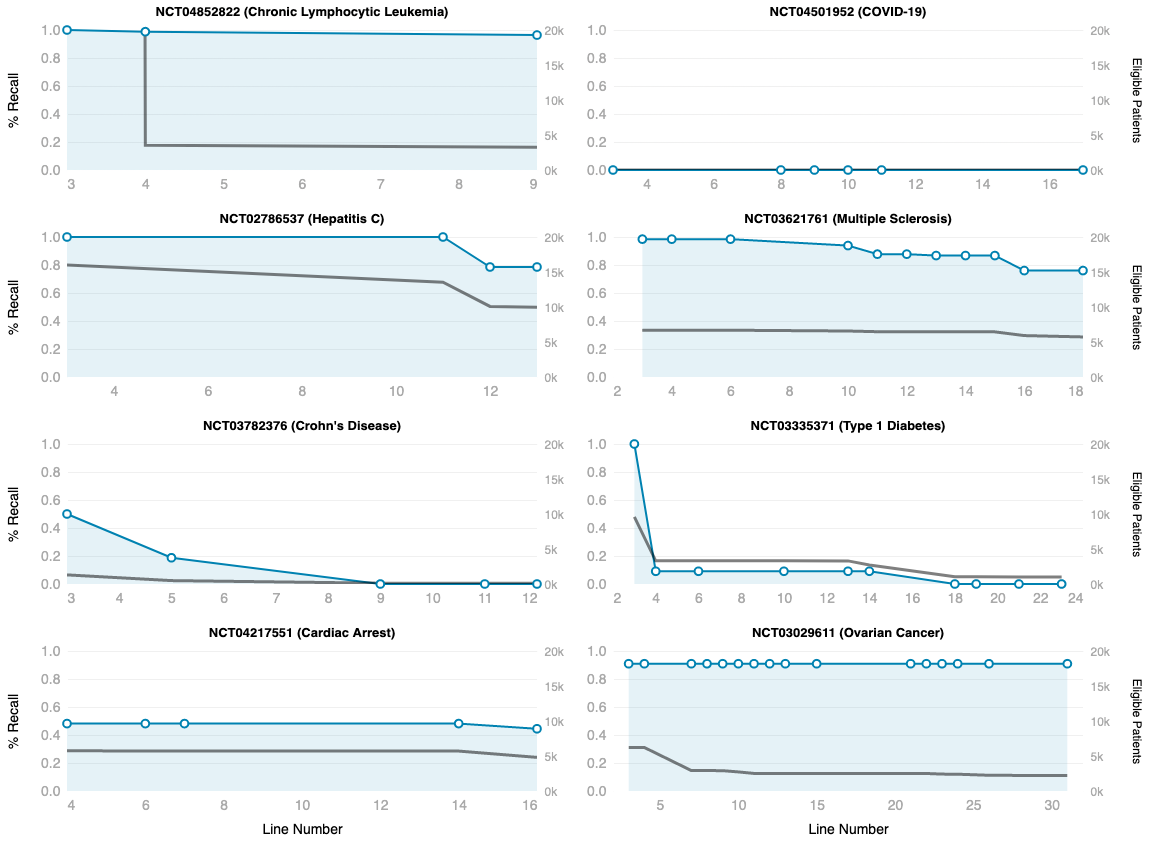
\includegraphics[scale=0.42]{figures/leafai_detail_results_longitudinal.png}  
\caption{}
\label{fig_leafai_results_longitudinal}
\end{figure}

\begin{table}[h!]
    \small
    \centering
    \def\arraystretch{1.4}
\begin{tabular}{l c c c c}
    \textbf{Condition} & \textbf{\# Criteria} & \textbf{Skipped - \newline No Patients} & \textbf{Skipped - \newline Not Computable} & \textbf{Fully Executed} \\
    \toprule
    Cl Lymphoma        & 4  & 0 (0\%)    & 0 (0\%)    & 4  (100\%)  \\
    Hepatitis C        & 8  & 0 (0\%)    & 4 (50\%)   & 4  (50\%)   \\
    Crohn's Disease    & 9  & 0 (0\%)    & 4 (44.4\%) & 5  (55.5\%) \\
    Cardiac Arrest     & 12 & 0 (0\%)    & 8 (66.6\%) & 4  (33.3\%) \\
    COVID-19           & 13 & 0 (0\%)    & 6 (46.1\%) & 7  (53.8\%) \\
    Multiple Sclerosis & 14 & 1 (7.1\%)  & 3 (21.4\%) & 10 (71.4\%) \\
    Type 1 Diabetes    & 18 & 2 (11.1\%) & 8 (44.4)   & 8  (44.4\%) \\
    Ovarian Cancer     & 25 & 2 (8\%)    & 9 (36\%)   & 14 (56\%)   \\
    \bottomrule
    \textbf{Total} & 103 & 5 (4.8\%) & 42 (40.7\%) & 61 (59.3\%)
\end{tabular}
    \caption{}
    \label{tbl_results_leafai_detail}
\end{table} 


\end{document}
    \caption{Statistics for each clinical trial evaluated by the LeafAI query engine and human programmer. The number of enrolled and matched patients were determined by cross-matching enrollments listed within our EHR. The \textit{Time} column indicates the number of hours the human programmer spent developing queries for each trial.}
    \label{tbl_results}
\end{table} 

Table \ref{tbl_results_leafai_detail} shows the number of criteria which were skipped by LeafAI. Of the 103 total criteria across all 8 studies, LeafAI executed queries for 61 (59.3\%) and skipped 5 (4.8\%) as it found no patients and 42 (40.7\%) because no computable concepts were found. 

\begin{table}[h!]
    \footnotesize
    \centering
    \def\arraystretch{1.4}
\begin{tabular}{l c c c c c}
    \textbf{Condition} & \textbf{\# Criteria} & \textbf{\# No Patients} & \textbf{\# Not Computable} & \textbf{\# Fully Executed} \\
    \toprule
    Cl Lymphoma        & 4  & 0 (0\%)    & 0 (0\%)    & 4  (100\%)  \\
    Hepatitis C        & 8  & 0 (0\%)    & 4 (50\%)   & 4  (50\%)   \\
    Crohn's Disease    & 9  & 0 (0\%)    & 4 (44.4\%) & 5  (55.5\%) \\
    Cardiac Arrest     & 12 & 0 (0\%)    & 8 (66.6\%) & 4  (33.3\%) \\
    COVID-19           & 13 & 0 (0\%)    & 6 (46.1\%) & 7  (53.8\%) \\
    Multiple Sclerosis & 14 & 1 (7.1\%)  & 3 (21.4\%) & 10 (71.4\%) \\
    Type 1 Diabetes    & 18 & 2 (11.1\%) & 8 (44.4)   & 8  (44.4\%) \\
    Ovarian Cancer     & 25 & 2 (8\%)    & 9 (36\%)   & 14 (56\%)   \\
    \bottomrule
    \textbf{Total}     & 103 & 5 (4.8\%) & 42 (40.7\%) & 61 (59.3\%)
\end{tabular}
    \caption{The LeafAI query engine's handling of eligibility criteria for each trial. The column \textit{No Patients} indicates the count of criteria which would, if executed, cause no patients to be eligible. The column \textit{Not Computable} indicates the count of criteria which LeafAI could not generate a query for, for various reasons. Both of these types of criteria were ignored by the system.}
    \label{tbl_results_leafai_detail}
\end{table} 

Figure \ref{fig_leafai_results_analysis} shows differences in query strategies for 4 trials between LeafAI and the human programmer. 

\begin{figure}[h!]
  \begin{center}
    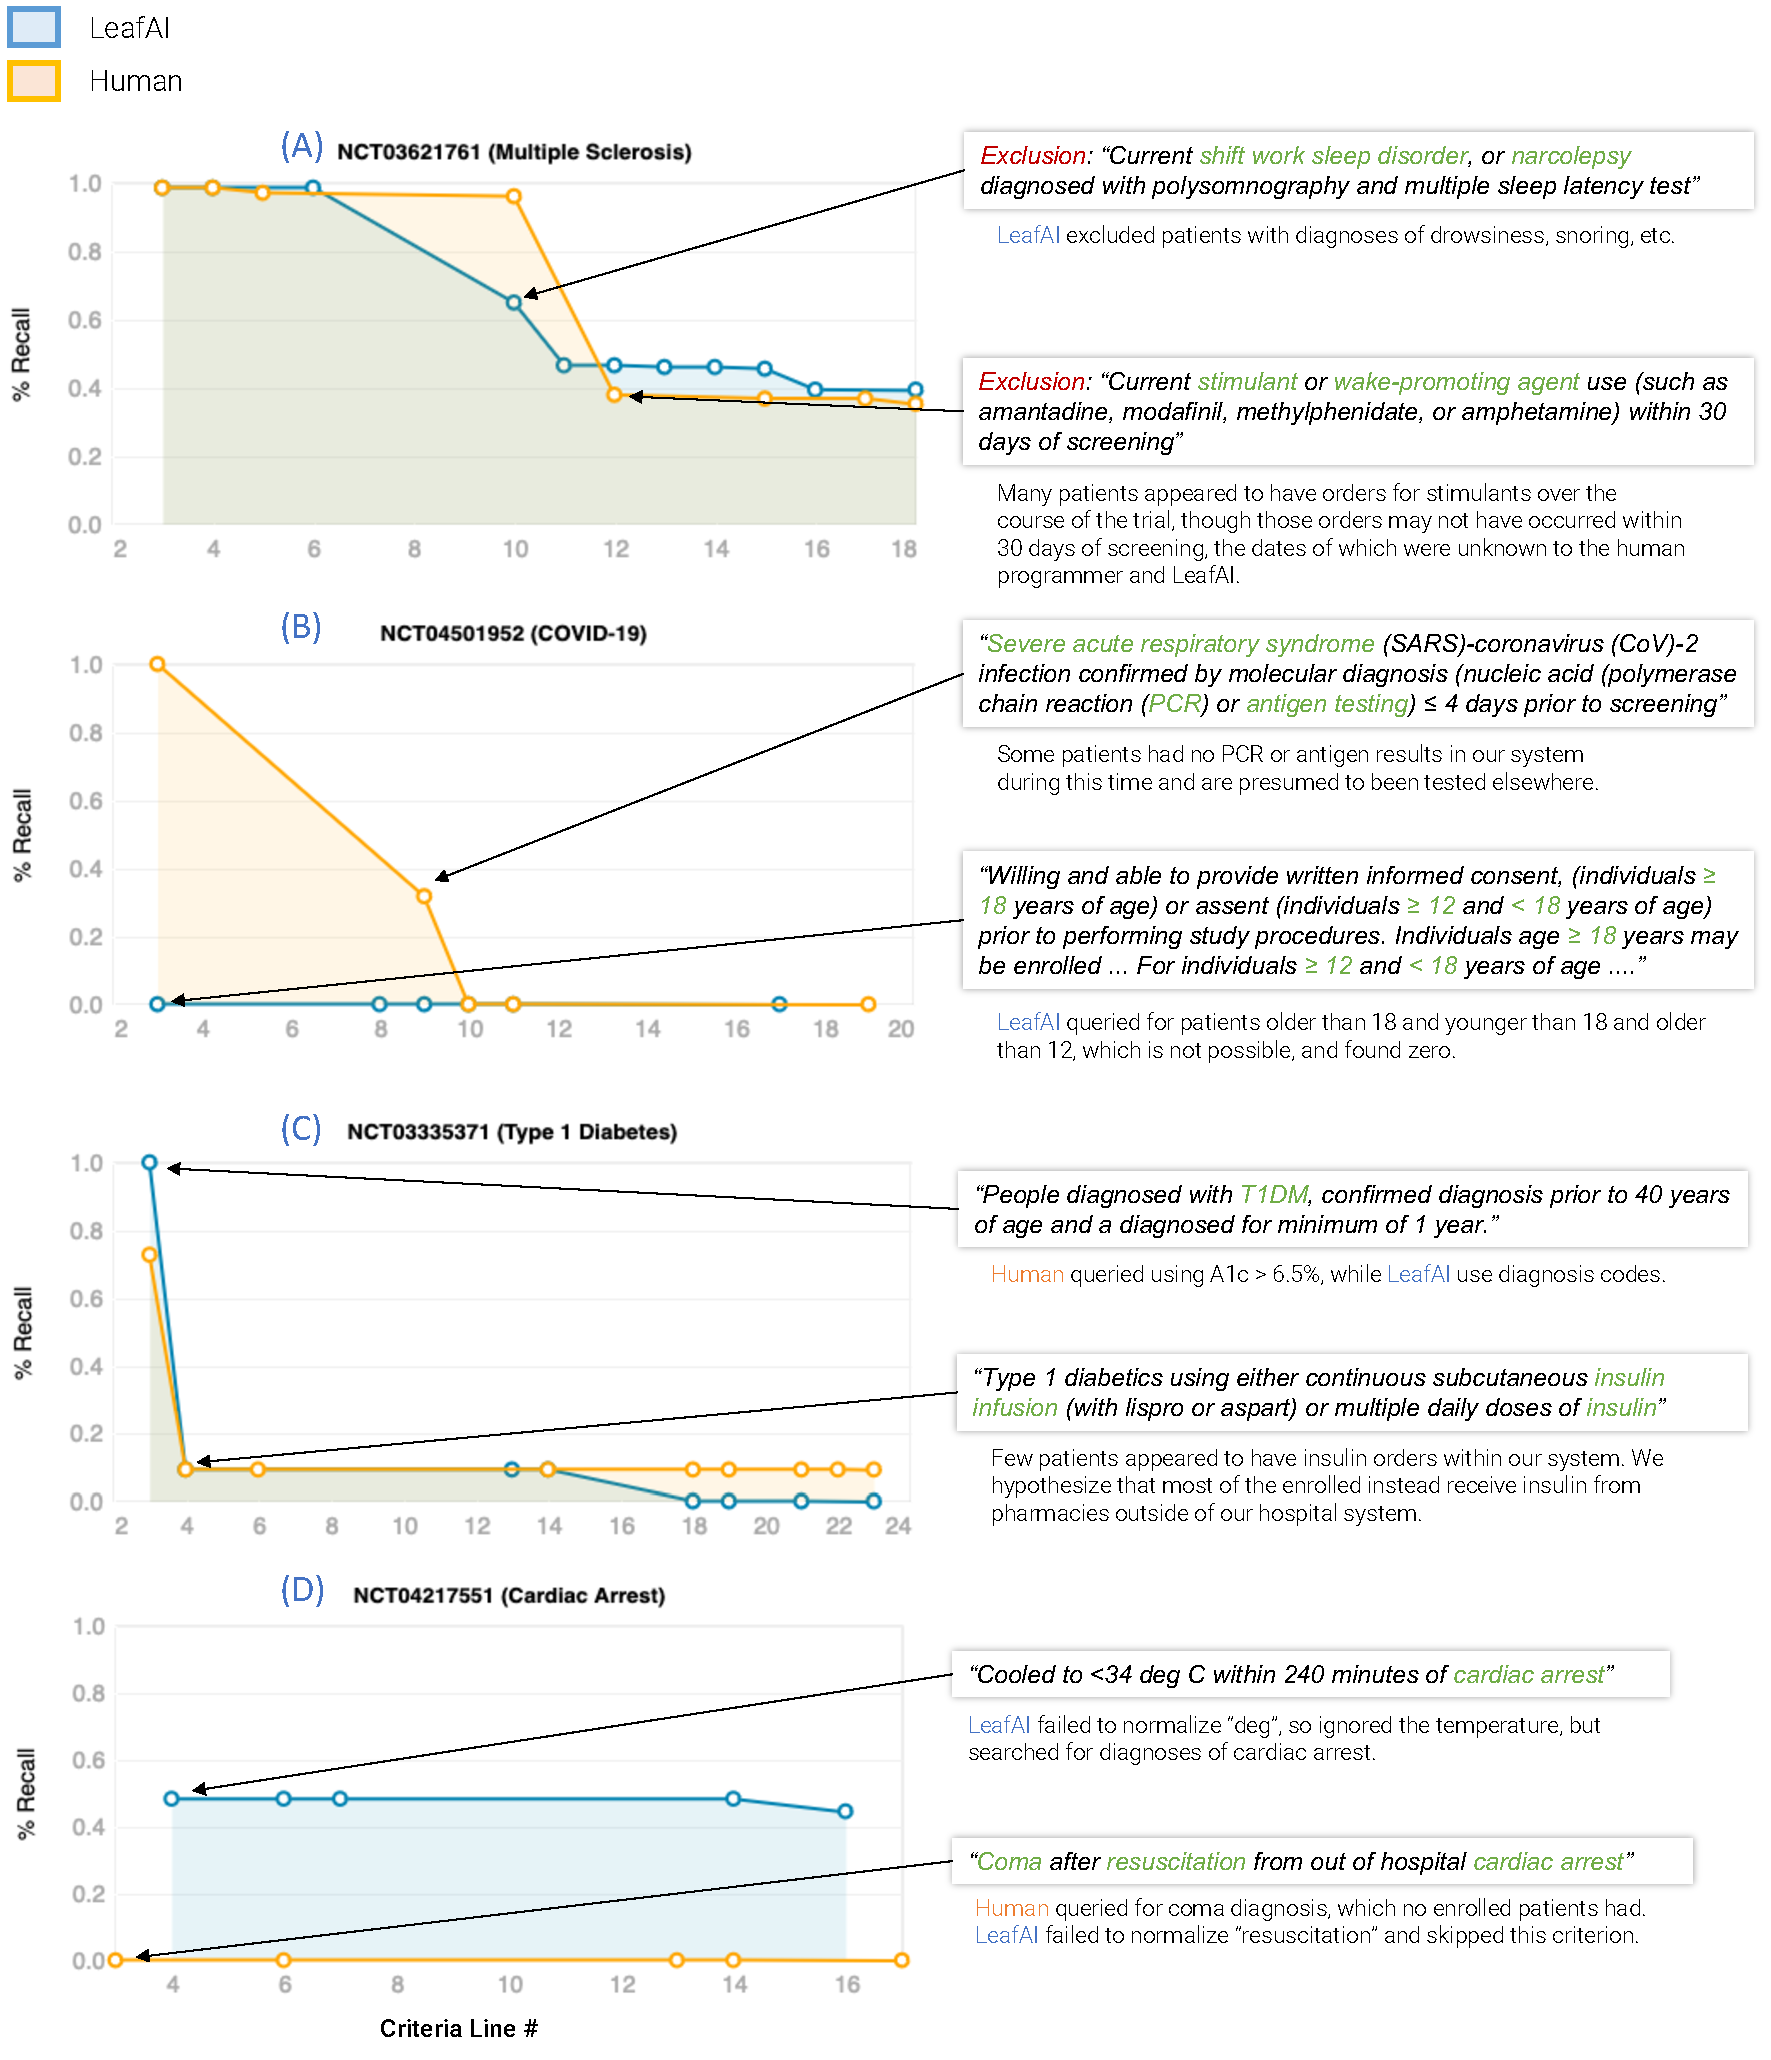
\includegraphics[scale=0.54]{Figures/7_query_generation/leafai_analysis.pdf}  
  \end{center}
  \caption{Longitudinal results listing patients found at each step in the query process for four trials illustrating data issues and differing query strategies between LeafAI and the human programmer. The blue line indicates recall for LeafAI and orange that of the human programmer. The X axis represents the line number within the free-text eligibility criteria. Dots indicate that a query was executed for a given line. On the right, boxes represent the text of a given eligibility criteria, with comments below discussing strategies and findings.}
  \label{fig_leafai_results_analysis}
\end{figure}

\section{Discussion}

Our results demonstrate that LeafAI is capable of rivaling the ability of a human programmer in identifying patients who are potentially eligible for  clinical trials. Indeed, in numerous cases we found LeafAI and the human programmer executing similar queries, such as for Hepatitis C (NCT04852822), Chronic Lymphocytic Leukemia (NCT04852822), MS (NCT03621761), and Diabetes Mellitus (NCT03029611), where both ultimately matched a similar number of patients.

One notable pattern we found is that LeafAI consistently finds a higher number of potentially eligible patients. We hypothesize that in many cases, LeafAI’s KB played a key role both in finding additional eligible patients. For example, in the MS trial, LeafAI searched for 11 different SNOMED codes related to MS (including MS of the spinal cord, MS of the brain stem, acute relapsing MS, etc.), while the human programmer searched for only one, and ultimately LeafAI found nearly 5 times the number of potentially eligible patients (4,891 versus 1,016). It is possible that the human programmer had a lower rate of false positives (and thus higher precision); this will be explored in a future analysis.  On the other hand, in the same trial, as can be seen in Figure \ref{fig_leafai_results_analysis} (A), given the exclusion criteria: "Current shift work sleep disorder, or narcolepsy diagnosed with polysomnography and multiple sleep latency", LeafAI’s KB unnecessarily excluded otherwise eligible patients by removing those with diagnosis codes for drowsiness, snoring, etc., as within the UMLS those are child concepts of sleep disorder (C0851578). The exclusion of these patients likely resulted in an approximately 40\% drop in recall at that stage compared to the human programmer, though ultimately both achieved similar recall (LeafAI: 39\% versus Human: 35\%).

Beyond performance as measured by recall, it is notable that the human programmer spent approximately 26 hours crafting queries for the 8 trials while LeafAI took only several minutes running on a single laptop. The time saved by using automated means such as LeafAI for cohort discovery may save health organizations significant time and resources.

\subsection*{Limitations}

This project has a number of limitations. First, while the 8 clinical trials we evaluated were randomly selected, we specifically restricted the categories of diseases from which trials were chosen and limited to trials with 30 or less lines of eligibility criteria, and thus our results may not generalize to other kinds of trials. Next, we evaluated our queries using an OMOP-based extract which did not contain the full breadth of data within our EHR. Had our experiments instead been conducted using our enterprise data warehouse (populated by our EHR), it is possible the human programmer would have achieved better results than LeafAI due to knowledge and experience in utilizing granular source data. For example, in the Cardiac Arrest clinical trial, the human programmer noted that data for use of cooling blankets is available in our EHR, but not in OMOP. It is not clear how LeafAI would perform were such data available. We further did not directly compare LeafAI to other NLP systems. While we considered evaluating another notable system, Criteria2Query \cite{yuan2019criteria2query}, as part of our baseline, we ultimately determined that it was inappropriate for our analysis as we aimed to review results longitudinally (i.e., line by line of criteria), a function which Criteria2Query does not perform. Last, the number of truly eligible patients within our institution for each trial is unknown, which hampers our ability to measure system performance. We used each trial’s known enrolled participants as our gold standard, but assume they are only a (possibly small) subset of those actually eligible.

\section{Conclusions}

This study introduced LeafAI, a NLP-based system leveraging deep learning and an integrated KB which can automatically generate queries for cohort discovery on virtually any clinical data model. Using an OMOP database representing the entire patient population of our institution, we demonstrated that LeafAI rivals the  performance of a human programmer in identifying eligible research candidates. As future work we will deploy LeafAI into the analytic tool box for our  research community, obtaining their feedback and iteratively improving the  tool.

\end{document}